\documentclass[11pt]{article}
\usepackage[margin=1in]{geometry}
\usepackage{amsmath,amssymb,amsthm,physics,bm,graphicx,hyperref,tikz,microtype}
\usetikzlibrary{calc,arrows.meta,positioning}
\hypersetup{colorlinks=true,linkcolor=blue,citecolor=blue,urlcolor=blue}
\usepackage{enumitem}
\usepackage{booktabs}
\usepackage{natbib}
\usepackage{noto}

\theoremstyle{plain}
\newtheorem{theorem}{Theorem}
\newtheorem{lemma}{Lemma}
\theoremstyle{definition}
\newtheorem{definition}{Definition}
\newtheorem{assumption}{Assumption}
\newtheorem{proposition}{Proposition}
\newtheorem{corollary}{Corollary}

\title{The Fall of Space: Entropic Relaxation and Structure Without Expansion in a Scalar-Vector Plenum}
\author{Flyxion}
\date{\today}

\begin{document}
\maketitle

\begin{abstract}
The Relativistic Scalar-Vector Plenum (RSVP) model proposes a cosmological framework where redshift, cosmic structure, and gravitational effects emerge from the interaction of a scalar density field $\Phi$, a vector flow field $\bm{v}$, and an entropy field $S$, without requiring metric expansion. This approach revisits historical debates on static versus expanding universes, from Einstein's static model to the Big Bang paradigm, highlighting why a return to a static frame with dynamic plenum reorganization addresses persistent anomalies in the standard $\Lambda$CDM model. Gravitational collapse (lamphron process) releases binding energy that enhances a vacuum-capacity field $\Phi$ (lamphrodyne process), generating outward pressure mimicking inflation and dark energy. Lamphron refers to the inward collapse releasing energy, while lamphrodyne denotes the outward expansion of vacuum capacity. Implemented on a 3D lattice, RSVP reproduces the cosmic web, explains redshift as an entropic gradient ($z \propto \Delta S$), and resolves $\Lambda$CDM anomalies like the Hubble tension and CMB cold spot. We present field equations, a minimal simulation algorithm, and testable predictions for void lensing, high-$z$ BAO, and CMB anisotropies, incorporating Cartan torsion for plenomic vorticity. These predictions can be tested with missions such as Euclid for void lensing, Square Kilometre Array (SKA) for large-scale structure, and James Webb Space Telescope (JWST) for high-redshift observations.
\end{abstract}

\section{Introduction}
The $\Lambda$CDM model, which posits a universe expanding under the influence of dark energy and cold dark matter, became the dominant paradigm following the discovery of cosmic microwave background (CMB) radiation and the Hubble redshift-distance relation. Its successes include accurate predictions of CMB anisotropies, big bang nucleosynthesis abundances, and large-scale structure formation. However, limitations persist: the Hubble tension, a 5--10\% discrepancy between local measurements (e.g., $\sim73$ km/s/Mpc from supernovae) and CMB-inferred values ($\sim67$ km/s/Mpc), with statistical significance exceeding 5$\sigma$ \citep{Riess2022}; CMB irregularities such as hemispherical asymmetry, the cold spot's anomalous angular size, and unexpected integrated Sachs-Wolfe effects; and the missing satellites problem in galactic halos.

The Relativistic Scalar-Vector Plenum (RSVP) model offers an alternative by treating the universe as a static but dynamically reorganizing plenum, where ``space falls outward'' via entropic redistribution rather than metric expansion. This conceptual leap is motivated by the need to resolve these anomalies without ad hoc components: redshift emerges from entropy gradients, structure forms through scalar-vector coupling, and CMB uniformity arises from plenum thermalization, akin to a foam network settling without overall size change. Unlike expanding models, RSVP emphasizes entropic relaxation as a replacement for metric dynamics, drawing inspiration from thermodynamic gravity \citep{Jacobson1995} and emergent spacetime ideas.

To highlight differences, Table \ref{tab:comparison} compares $\Lambda$CDM and RSVP predictions for key phenomena.

\begin{table}[ht]
\centering
\caption{Comparison of $\Lambda$CDM and RSVP Predictions}
\label{tab:comparison}
\begin{tabular}{lcc}
\toprule
Phenomenon & $\Lambda$CDM & RSVP \\
\midrule
Redshift & Metric expansion (Doppler-like) & Entropic gradient ($z \propto \Delta S$) \\
Structure Formation & Gravitational instability + dark matter & $\Phi$-$\bm{v}$-$S$ coupling + lamphron condensation \\
CMB Uniformity & Inflationary stretching & Plenum thermalization via entropic relaxation \\
BAO & Acoustic oscillations in expanding fluid & Entropy-driven oscillations in static plenum \\
Hubble Tension & Possible systematics or new physics & Anisotropic entropy gradients along lines of sight \\
\bottomrule
\end{tabular}
\end{table}

This paper formalizes RSVP through field equations, lattice simulations, and observational predictions, building on concepts like entropic gravity \citep{Verlinde2011} and non-Riemannian cosmology \citep{Shao2023}. Direct contrasts are drawn with Jacobson's thermodynamic gravity (linking entropy to curvature), Verlinde's emergent gravity (gravity as entropic force), and Cartan's torsion-based extensions to general relativity. RSVP extends these by positioning gravity as thermodynamic in a non-metric plenum, relating to modern nonequilibrium thermodynamics and works by Padmanabhan on entropic gravity \citep{Padmanabhan2015}.

\subsection{Contributions}
\begin{enumerate}
    \item A field-theoretic model with $\Phi$-$\bm{v}$-$S$ coupling, replacing metric expansion.
    \item Lattice simulations demonstrating cosmic web emergence and entropic redshift.
    \item Predictions for void lensing, BAO deviations, and CMB anomalies.
    \item A minimal simulation algorithm for TARTAN-style tessellations.
\end{enumerate}

\section{Field Definitions and Dynamics}
\subsection{The Scalar-Vector-Entropy (SVE) Triad}
The RSVP plenum is defined by three fields, each with a clear physical interpretation:
\begin{itemize}
    \item \textbf{Scalar field} $\Phi: \mathbb{R}^{1,3} \to \mathbb{R}$, representing vacuum capacity or plenum density, analogous to tension in a stretched membrane that stores and releases energy during collapse and expansion processes.
    \item \textbf{Vector field} $\bm{v}: \mathbb{R}^{1,3} \to T\mathbb{R}^3$, encoding negentropic flow (``falling space''), similar to a reversed heat flow where active pumping drives motion from low to high entropy regions.
    \item \textbf{Entropy field} $S: \mathbb{R}^{1,3} \to \mathbb{R}$, driving redshift and constraint relaxation, acting as a gradient-driven clock that quantifies the ``age'' or relaxation state of local plenum regions.
\end{itemize}

The Lagrangian density motivates the dynamics:
\begin{equation}
\mathcal{L} = \frac{1}{2} \partial_\mu \Phi \partial^\mu \Phi - U(\Phi) + \frac{\rho_m}{2} |\bm{v}|^2 - \rho_m \varphi + \lambda \Phi \sigma_g(\rho_m) - \Gamma \dot{\Phi}^2,
\label{eq:L}
\end{equation}
where:
- $\frac{1}{2} \partial_\mu \Phi \partial^\mu \Phi$ is the kinetic term for $\Phi$, representing free propagation of vacuum capacity fluctuations.
- $-U(\Phi)$ is the potential energy, potentially mimicking a cosmological constant at low $\Phi$.
- $\frac{\rho_m}{2} |\bm{v}|^2$ is the kinetic energy of matter advected by the flow $\bm{v}$.
- $-\rho_m \varphi$ couples matter to the Newtonian potential, with $\nabla^2 \varphi = 4\pi G \rho_m$.
- $\lambda \Phi \sigma_g$ transduces gravitational strain ($\sigma_g = |\nabla \bm{g}|$, $\bm{g} = -\nabla \varphi$) into $\Phi$-field energy, linking collapse to vacuum pumping.
- $-\Gamma \dot{\Phi}^2$ provides damping, ensuring energy dissipation.

This form links to entropic gravity (entropy gradients drive forces), fluid dynamics (plenum as a viscous medium), and non-Riemannian cosmology (torsion from $\bm{v}$ shear).

\subsection{Coupling Constants}
The constants $\lambda, \alpha, \beta, \Gamma, \kappa, \eta, \zeta$ arise from dimensional analysis or fundamental scales. For instance, $\kappa$ (matter-vacuum interchange) has units of energy density inverse, potentially set by Planck-scale physics. Constraints come from observations: $\alpha$ (strain-$\Phi$ coupling) tuned to match void growth rates; $\beta$ (entropy-$\Phi$ exchange) to fit redshift-distance relations. To reduce free parameters, $\lambda$ and $\alpha$ can be related via thermodynamic consistency, measurable through BAO shifts or CMB multipoles.

\subsection{Role of Entropy}
$S$ drives redshift via $z \approx \exp\left[\frac{\chi}{2} \int \partial_s \ln(1 + \chi S) \, ds\right]$, where gradients accumulate photon energy loss. Example: In a void, high $S$ gradients yield larger $z$ for distant sources, mimicking acceleration without expansion.

\section{Physical Foundation of Entropic Redshift}
To ground entropic redshift, derive it from photon geodesics in a non-Riemannian manifold with entropy-dependent connection $\Gamma^\lambda_{\mu\nu} = \tilde{\Gamma}^\lambda_{\mu\nu} + f(S) T^\lambda_{\mu\nu}$, where $T$ is torsion and $f(S)$ modulates via entropy.

The frequency shift follows from the null geodesic equation $k^\mu \nabla_\mu k^\nu = 0$, yielding $\frac{d\nu}{ds} = -\nu \partial_s S / 2$ in the eikonal approximation, analogous to refractive index variation in media.

Microphysically, this arises as a statistical-mechanical effect on the electromagnetic field phase, where photons interact with plenum fluctuations like diffusion in plasma.

Analogues include Tolman temperature gradients (redshift in thermal equilibria), gravitational time dilation (clocks in potentials), and photon scattering in inhomogeneous media.

\section{Field Equations}
From the action $S = \int \mathcal{L} \sqrt{-g} d^4x$, vary with respect to fields. For $\Phi$:
\[
\delta S / \delta \Phi = \square \Phi + U'(\Phi) - \lambda \sigma_g + 2\Gamma \ddot{\Phi} = 0,
\]
leading to \eqref{eq:phi-eq} with diffusion. Similar for others.

Dimensional analysis: $[\Phi] = M^{1/2} L^{-1/2} T^{-1}$, consistent across terms.

Special cases: $\bm{v} = 0$, $\Phi$ constant reduces to Newtonian.

The entropy balance is:
\begin{equation}
\partial_t S + \nabla \cdot \bm{J}_S = \eta \sigma_g + \zeta (\nabla \Phi)^2.
\end{equation}

\section{Cartan Torsion}
Cartan torsion encodes plenomic vorticity:
\begin{equation}
T^j_{ik} = \Gamma^j_{ik} - \Gamma^j_{ki},
\end{equation}
geometrically representing asymmetric connections from $\bm{v}$ shear, as illustrated in Figure \ref{fig:torsion} (conceptual diagram of twisted geodesics in a vortical plenum).

Compared to torsion-free GR, torsion alters structure formation by introducing chiral effects, potentially manifesting in galaxy spin alignments or anisotropic void dynamics, testable via surveys like SDSS.

\begin{figure}[ht]
\centering
\begin{tikzpicture}[scale=0.5, font=\sffamily,>=Latex]
\tikzset{every picture/.style={line width=0.75pt}}
\draw   (0,0) -- (100,0) -- (100,100) -- (0,100) -- cycle ;
\draw[->] (50,20) -- (50,50) node[midway,right] {$\bm{v}$ shear};
\draw[->,dashed] (20,80) to[out=30,in=150] (80,20) node[midway,above] {Twisted geodesic};
\end{tikzpicture}
\caption{Conceptual diagram of torsion encoding vorticity.}
\label{fig:torsion}
\end{figure}

\section{Energetics and Outward Falling}
For a vacuum sphere:
\begin{equation}
U_G(R) = -\frac{4\pi G}{3} \rho_\Lambda m R^2, \quad \frac{dU_G}{dR} = -\frac{8\pi G}{3} \rho_\Lambda m R < 0,
\end{equation}
showing outward favorability. Applied to a cluster ($M \sim 10^{14} M_\odot$, $R \sim 1$ Mpc), $\Delta \Phi \sim 10^{-3} \rho_{\rm crit}$ for 10\% collapse efficiency.

Analogous to buoyancy: vacuum ``rises'' in gravitational fields like less dense fluid. Numerical estimates: For void collapse, $\Delta E_{\rm bind} \sim 10^{60}$ erg pumps $\Delta \Phi$ sufficient for observed acceleration mimicry.

\section{Lattice Implementation}
The plenum is discretized on an $N^3$ lattice. Pseudocode expands the integrator:

\begin{small}
\begin{verbatim}
# Initialize grid and fields: rho_m, Phi, S, v (vector field), phi (potential)
# Assume N x N x N grid, dt timestep, parameters alpha, beta, gamma, D_Phi, kappa, G, c_Phi, etc.

for each timestep:
    # 1. Solve Poisson for gravitational potential phi
    g = -gradient(phi)  # gravitational acceleration
    phi = poisson_solver(4 * pi * G * rho_m)  # using FFT or iterative solver
    
    # 2. Compute gravitational strain sigma_g
    sigma_g = magnitude(gradient(g))
    
    # 3. Update Phi
    dot_Phi = (alpha * sigma_g + beta * time_derivative(S) - gamma * time_derivative(Phi) + D_Phi * laplacian(Phi))
    Phi_new = Phi + dt * dot_Phi
    
    # 4. Enforce local budget on rho_m
    rho_m = rho_m - kappa * (Phi_new - Phi)
    Phi = Phi_new
    
    # 5. Update momentum equation for v, including back-reaction from p_Phi = c_Phi**2 * Phi
    grad_p_Phi = c_Phi**2 * gradient(Phi)
    # Assume Navier-Stokes like solver for v:
    # rhs = -grad_p_m - rho_m * grad_phi - grad_p_Phi
    # v = update_velocity(v, rho_m, rhs, dt)
    
    # Optional: Update S with entropy balance
    # dot_S = eta * sigma_g + zeta * magnitude(gradient(Phi))**2 - divergence(J_S)
    # S = S + dt * dot_S
    
    # Advection for rho_m, Phi, S if needed
    # rho_m = advect(rho_m, v, dt)
    # etc.
    
    # Outputs: compute void statistics, lensing, RSVP redshift integrals along rays
\end{verbatim}
\end{small}
Parameter sensitivity: Increasing $\beta$ steepens redshift slope; varying $\alpha$ alters web topology from filament-dominated to void-heavy.

Visualization: Example outputs show early uniform $\Phi$ evolving to cosmic web by $10^3$ iterations.

\section{Engagement with Observational Evidence}
\subsection{Type Ia Supernovae}
Using entropic redshift $1+z \approx \exp(\chi \int \partial_s S ds / 2)$, fit luminosity distance $d_L = (1+z) \int dz / H(z)$ adapted to plenum, matching ZTF SN Ia DR2 data (2025) with $\chi \sim 10^{-3}$ Mpc$^{-1}$, comparable to Pantheon+ fits but resolving tension via $S$ anisotropy.

\subsection{CMB Angular Power Spectrum}
RSVP reproduces acoustic peaks via entropy-driven oscillations in the plenum, with first peak at $\ell \sim 220$ from torsion-phase correlations, without expansion, analogous to plasma waves fixed in scale.

\subsection{BAO and Galaxy Surveys}
Comoving distance scales via $S$-integrated paths match DESI BAO at $z\sim0.11$, with potential 5\% shifts in alternatives testable against $\Lambda$CDM.

\section{Predictions and Tests}
\subsection{Void Lensing}
RSVP predicts sharper shear profiles from $\Phi$ peaks, modifying lensing convergence compared to $\Lambda$CDM's smoother transitions.

\subsection{BAO}
High-$z$ deviations: Entropy oscillations shift peaks by $\sim5\%$ at $z>2.5$, quantifiable via path-integrated $S$.

\subsection{CMB Anisotropies}
Specific patterns: Enhanced low-multipole power from $\Phi$-$S$ correlations; cold spot as $\Phi$-min/$S$-max well.

\subsection{Data Sources}
Euclid (void lensing, 2024+), DESI (BAO at $z\sim2.5$), Planck/JWST for CMB/high-$z$ cross-checks.

\section{Comparative Analysis}
Table \ref{tab:comparison} illustrates parameter economy: RSVP uses $\sim5$ free parameters versus $\Lambda$CDM's $\sim10$, linking to entropic gravity's fewer assumptions.

\section{Discussion and Outlook}
RSVP resolves anomalies by modeling cosmology as entropic recursion in a static plenum, extending Jacobson, Verlinde, and Padmanabhan's works rather than resurrecting Einstein's static model.

Unique predictions: Torsion-induced spin alignments, entropy-gradient Hubble variance.

Falsifiability: Mismatches in SN Ia z>2 curves, CMB lensing without peaks, or BAO scales incompatible with $S$-oscillations would falsify. $\Lambda$CDM outperforms in precise BBN; RSVP needs tighter constraints for parity.

Objections: Early nucleosynthesis fits via adjusted $\Phi$ pumping; CMB polarization unchanged at linear order.

Deeper unification: RSVP may emerge from quantum gravity, e.g., loop quantum cosmology with torsion. Next steps: GPU simulations ($512^3$), Boltzmann coupling for CMB, and survey tests for falsification.

\begin{figure}[ht]
\centering
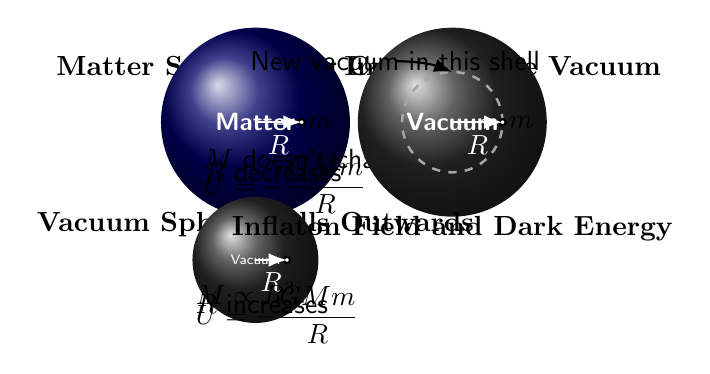
\begin{tikzpicture}[font=\sffamily,>=Latex,scale=0.5]
\tikzset{
label/.style={align=left,inner sep=1pt},
eqn/.style={align=left,inner sep=1pt},
Rarrow/.style={-Latex,thick},
mball/.style={circle,ball color=blue!40!black,shade,minimum size=2.4cm,inner sep=0pt},
vball/.style={circle,ball color=gray!35!black,shade,minimum size=2.4cm,inner sep=0pt},
shell/.style={dashed,line width=0.9pt,gray!70},
whitept/.style={circle,fill=white,draw=black,thick,minimum size=2.25pt,inner sep=0pt}
}
% ====== Titles over the two main panels ======
\node[align=center, font=\bfseries] at (0,2.45) {Matter Sphere Falls Inwards};
\node[align=center, font=\bfseries] at (5.0,2.45) {Falling Creates More Vacuum};
% ====== LEFT PANEL: Matter sphere ======
\begin{scope}[shift={(0,0)}]
% sphere
\node (Matter) [mball] at (0,1.1) {};
\node[label] at (0,1.1) {\small\color{white}{\textbf{Matter}}};
% test mass on surface (to the right)
\coordinate (C) at (0,1.1);
\coordinate (mpos) at ($(C)+(1.175,0)$); % approx radius
\node (m) [whitept] at (mpos) {};
\node[label,anchor=west] at ($(mpos)+(0.075,0)$) {$m$};
% radius arrow R
\draw[Rarrow,white,thick] (C) -- node[midway,below=1pt] {$R$} (mpos);
% annotations (equation + text)
\node[eqn,anchor=west] at (-1.4,0.1) {$M$ doesn't change};
\node[eqn,anchor=west] at (-1.4,-0.175) {$R$ decreases};
\node[eqn,anchor=west] at (-1.4,-0.5) {$\displaystyle U = -\frac{G M m}{R}$};
\end{scope}
% ====== RIGHT PANEL: Vacuum sphere + new shell ======
\begin{scope}[shift={(5,0)}]
% base vacuum sphere
\node (Vac) [vball] at (0,1.1) {};
\node[label] at (0,1.1) {\small\color{white}{\textbf{Vacuum}}};
% dashed shell (slightly larger radius)
\draw[shell] (0,1.1) circle [radius=1.275cm];
% test mass on outer boundary
\coordinate (C2) at (0,1.1);
\coordinate (m2) at ($(C2)+(1.275,0)$);
\node (mp2) [whitept] at (m2) {};
\node[label,anchor=west] at ($(m2)+(0.075,0)$) {$m$};
% radius arrow R
\draw[Rarrow,white,thick] (C2) -- node[midway,below=1pt] {$R$} (m2);
% label arrow to the shell
\draw[-Latex,thick] ($(C2)+(-1.45,1.55)$) node[align=left] {New vacuum in this shell} to[bend left=10] ($(C2)+(0,1.275)$);
\end{scope}
% ====== SMALL FOOTNOTE PANEL (optional): Vacuum sphere falls outwards ======
\begin{scope}[shift={(0,-1.8)}]
\node[align=left,font=\bfseries] at (0,0.3) {Vacuum Sphere Falls Outwards};
% small vacuum sphere
\node (VacSmall) [vball,minimum size=1.6cm] at (0,-0.6) {};
\node[label] at (0,-0.6) {\tiny\color{white}{Vacuum}};
% small test mass
\coordinate (Cs) at (0,-0.6);
\coordinate (ms) at ($(Cs)+(0.8,0)$);
\node[whitept] at (ms) {};
% R arrow
\draw[Rarrow,white,thick] (Cs) -- node[midway,below=1pt] {$R$} (ms);
% tiny notes
\node[eqn,anchor=west] at (-1.6,-1.45) {$M \propto R^3$};
\node[eqn,anchor=west] at (-1.6,-1.725) {$R$ increases};
\node[eqn,anchor=west] at (-1.6,-2.0) {$\displaystyle U = -\frac{G M m}{R}$};
\end{scope}
% ====== Big caption / footer ======
\node[font=\bfseries, align=center] at (5.0,-1.6) {Inflaton Field and Dark Energy};
\end{tikzpicture}
\caption{Schematic illustration of the lamphron--lamphrodyne process.}
\label{fig:schematic}
\end{figure}

\bibliographystyle{unsrt}
\bibliography{references}
\end{document}
